\section{Properties of Hamiltonian dynamics}



\section{Microcanonical averages}
Our aim in this section will be to describe methods to sample microcanonical averages. We will always consider microcanonical averages as ergodic averages under Hamiltonian trajectories.
To justify this approach, we should make sure that the microcanonical measure is invariant under the Hamiltonian dynamics. Indeed, this is the case:

The Hamiltonian dynamics \eqref{eq:hamiltonian_dynamics} rewrites in matrix form, writing $X_t=(q_t,p_t)$:

\begin{equation}\label{eq:hamiltonian_dynamics_matrix_form} \text d X_t=J\nabla H(X_t)\dt,\end{equation}
where $J$ is the symplectic matrix

$$J = \begin{pmatrix}
    0_{dN} & \Id_{dN}\\ -\Id_{dN} & 0_{dN}.
\end{pmatrix}$$
This will be useful to investigate properties of the Hamiltonian dynamics.
Applying the chain rule to any smooth function $\varphi: \cLs \mapsto \R$, we obtain
        $$ \text d \varphi(X_t)= \text d X_t^{\intercal} \nabla \varphi(X_t)=(J \nabla H(X_t))^\intercal \nabla \varphi(X_t)\dt=(\nabla_p H \cdot \nabla_q - \nabla_q H \cdot \nabla_p)\varphi(X_t)\dt$$
        This motivates the following.
        \begin{definition}[Generator of the Hamiltonian dynamics]
            We define the generator associated with the Hamiltonian dynamics to be the operator $\cL_{\text{H}}$ defined on smooth functions by
        \begin{equation}
            \label{eq:hamiltonian_generator}
            \cL_{\mathrm{ham}}\varphi=(\nabla_p H \cdot \nabla_q - \nabla_q H \cdot \nabla_p)\varphi=\left(J\nabla H\right)^\intercal \nabla \varphi
        \end{equation}
    \end{definition}
    We can split the generator as the sum of two elementary operators,
    $$\cLham=A+B,$$
    with
    \begin{equation}
        \label{eq:Lham_splitting}
        A=\left(M^{-1}p\right)\cdot \nabla_q \qquad B=-\nabla V(q)\cdot \nabla_p.
    \end{equation}
    The generator allows us to quantify the rate of change of an observable $\varphi$ under the evolution of the system. If we define, for $t\geq 0$, the evolution operators 
    $$P_t \varphi (q_0,p_0) = \varphi(\Phi_t(q_0,p_0)),$$
where $\Phi$ is the flow associated with the Hamiltonian dynamics, that is the collection of maps $(\Phi_t)_{t\geq 0}$, defined by
    $\Phi_t (q_0,p_0) = (q_t,p_t)$, the solution to \eqref{eq:hamiltonian_dynamics} with initial conditions  $(q_0,p_0)$, then we have formally:

    $$ \frac \partial{\partial t} P_t \varphi (q,p)= \partial_t \varphi(q_t,p_t)= \cLham \varphi(q_t,p_t)=\cLham P_t \varphi(q,p)=P_t\cLham \varphi(q,p).$$
    Applying $\cLham$ to $H$ immediately gives the following result.
\begin{prop}[Energy conservation]
    \begin{equation}
    \label{eq:energy_conservation} \text d H(X_t)=0
    \end{equation}
\end{prop}
This relation expresses the fact that the Hamiltonian is invariant under the flow of \eqref{eq:hamiltonian_dynamics}. This, in turn, is the mathematical translation of the physical principle of conservation of energy.
Using the fact that the Hamiltonian flow field is divergence-free,
\begin{equation}
        \label{eq:hamiltonian_flow_divergence_free}
        \mathrm{div}\left(J\nabla H\right)=\mathrm{div}_q\left(\nabla_p H\right)-\mathrm{div}_p\left(\nabla_q H\right)=0,
\end{equation}
one can show the following property, famously known as Liouville's theorem.
\begin{prop}[Conservation of volume]
    For any measurable set $D\subset \mathcal E$, we have
    \begin{equation}
        \label{eq:conservation_of_volume}
        |\Phi_t(D)|=|D|.
    \end{equation}
\end{prop}

\begin{definition}[Symplecticity]
    A mapping $\varphi$ from $\R^{2d}$ to itself is said to be symplectic on some open set $U\subset \R^{2d}$ if it is $C^1$ and if, for all $(q,p)\in U$,
    \[\nabla \varphi^\intercal J\nabla \varphi=J,\]
    where $\nabla \varphi$ is the Jacobian matrix of $\varphi$ \eqref{eq:jacobian}.
\end{definition}

\begin{prop}
    For any $t\in \R$, the Hamiltonian flow $Phi_t$ is symplectic.
\end{prop}
Consider the momentum-reversing map

\begin{equation}
    \label{eq:momentum_reversing}
    \cR(q,p)=(q,-p)
\end{equation}
We then have the following time symmetry property.
\begin{prop}[Time symmetry]
    \begin{equation}
        \Phi_t \circ \cR \circ \Phi_t=\Id
    \end{equation}
\end{prop}

\begin{remark}
    \label{rem:non_separable_hamiltonian}
    The property \eqref{eq:energy_conservation} is only due to the form of $J$, and not to the specific expression for $H$.
    Thus any $H$, we may consider any dynamics of the form \eqref{eq:hamiltonian_dynamics_matrix_form}, to devise a dynamical system whose orbits are restricted to the level set $H^{-1}\{H(q_0,p_0)\}$.\\
    Conversely, given a differential dynamical system, if through a change of coordinates one is able to write the system under this form, one has found a conservation law.
\end{remark}

    An important remark is that if one considers each part of \eqref{eq:Lham_splitting} as a generator in itself, the corresponding dynamics is analytically solvable.
    \begin{remark}
        \label{rem:Lham_splitting_semigroups}
        Consider the two dynamics defined by
        \begin{equation}
            \label{eq:Lham_splitting_dynamics}
            \left\{\begin{aligned}
                &\dif q_t^A=M^{-1}p_t^A\dif t, &\dif p_t^A=0,\\
                &\dif q_t^B=0, &\dif p_t^B=-\nabla V(q_t^B)\dif t.
            \end{aligned}\right.
        \end{equation}
        These are easily solved, namely
        \begin{equation}
            \label{eq:Lham_splitting_dynamics_solved}
            \left\{\begin{aligned}
                &\left(q_t^A,p_t^A\right)=\left(q_0^A+tp_0^A,p_0^A\right),\\
                &\left(q_t^B,p_t^B\right)=\left(q_0^B,p_0^B-tV\left(q_0^B\right)\right).
            \end{aligned}\right.
        \end{equation}
        Moreover, these evolutions are of Hamiltonian form, with Hamiltonians corresponding respectively to the kinetic part and the configurational part only, and have corresponding generators $A$ and $B$.
        We denote by $\left(\Phi^A_t\right)_{t\geq 0}$ and $\left(\Phi^B_t\right)_{t\geq 0}$ their respective flows. This splitting property will prove useful in constructing numerical schemes for both Hamiltonian and stochastic dynamics.
    \end{remark}

    \subsection{Numerical schemes for Hamiltonian dynamics}

    It is impossible, except for a very restricted class of systems, which do not occur in practical settings anyhow, to analytically integrate Hamilton's equation \eqref{eq:hamiltonian_dynamics}. For this reason, one must revert to numerical schemes, which we may interpret as discrete approximations of the Hamiltonian flow.
    More precisely, for a fixed timestep $\Delta t$, if we possess an approximation of the flow 
    \[\tilde\Phi_{\Delta t}\approx\Phi_{\Delta t},\]
    we will deduce approximations of the evolution
    \begin{equation}\label{eq:discrete_dynamics}(q^n,p^n)\defeq \tilde\Phi_{\Delta t}^n(q_0,p_0)\approx (q_{n\Delta t},p_{n\Delta t}),\end{equation}
    which can then be used as sample points for the computation of empirical averages, discrete counterparts to the ergodic averages \eqref{eq:ergodic_averages},
    \begin{equation}
        \label{eq:discrete_ergodic_averages}
        \frac 1n\sum_{k=0}^n \varphi(q^n,p^n).
    \end{equation}
    In most common applications, the aim is to approximate the exact solution of an evolution equation as precisely as possible over a given time domain.
    In the case of molecular dynamics, however, the time domain is usually very large, because simulating long trajectories is a requirement to ensure that a representative portion of phase space is explored. As a consequence, it is in practice impossible to obtain precise solutions over a long time, because of the evolution's sensitivity to the initial conditions. 
    Furthermore, one does not even care about the exact evolution, since the dynamics are merely used as a sampling device. Instead, one key requirement is that the dynamics stay on or close to the constant Hamiltonian manifold associated with the initial conditions. It can be shown through eigenanalysis that for simple linear systems, this requirement is not satisfied by standard ODE numerical methods such as the explicit and implicit Euler schemes, or the RK4 method, for which the energy may explode or implode geometrically.
    This has the practical effect that for reasonably sized atomic systems, numerical instabilities render the simulations nonsensical after only a few time steps, a far cry from what is needed to obtain good estimates.
    One must then devise dedicated numerical methods, guided by the aim to preserve qualitative properties of the Hamiltonian evolution. It turns out that splitting schemes, based on operator splitting approximations of the Hamiltonian evolution operator over one timestep, preserve crucial qualitative properties of the Hamiltonian evolution.
    Let us fix a timestep $\Delta t>0$. Numerical schemes aim to approximate the flow $\Phi_{\Delta t}$. Splitting schemes rely on the splitting property \eqref{eq:Lham_splitting_dynamics_solved} to construct computable approximations
    \[\Phi_{\Delta t}\approx \Phi^{G_k}_{\Delta t_k}\circ \dotsm \circ \Phi^{G_1}_{\Delta t_1},\]
    where $G_i\in\{A,B\}$ for all $i$. We will be considering three schemes, the simplest of which are the symplectic Euler schemes.
    
    The symplectic Euler schemes are defined by the following update equations.
    
    \begin{equation}\label{eq:symplectic_euler_A}
    \left\{\begin{aligned}
         p^{n+1} &=p^n -\nabla V(q^n)\Delta t\\
         q^{n+1} &=q^n + M^{-1}p^{n+1}\Delta t
    \end{aligned}\right.
    \end{equation}

    \begin{equation}\label{eq:symplectic_euler_B}
        \left\{\begin{aligned}
             q^{n+1} &=q^n +M^{-1}p^n\Delta t\\
             p^{n+1} &=p^n - \nabla V(q^{n+1})\Delta t
        \end{aligned}\right.
    \end{equation}

    These correspond respectively to the splitting approximations 
    \[\Phi_{\Delta t}\approx \Phi_{\Delta t}^A\circ\Phi_{\Delta t}^B\defeq \Phi_{\Delta t}^{BA}\]
    and
    \[\Phi_{\Delta t}\approx \Phi_{\Delta t}^B\circ\Phi_{\Delta t}^A\defeq \Phi_{\Delta t}^{AB}.\]
    
    The velocity Verlet scheme is based on the splitting
    \[\Phi_{\Delta t}\approx \Phi_{\Delta t/2}^B\circ\Phi_{\Delta t}^A\circ\Phi_{\Delta t/2}^B\defeq \Phi_{\Delta t}^{BAB}.\]
    Its update equation is given by
    \begin{equation}\label{eq:verlet}
        \left\{\begin{aligned}
             p^{n+\frac12} &=p^n -\frac{\Delta t}{2}\nabla V(q^n)\\
             q^{n+1} &=q^n + \Delta t M^{-1}p^{n+\frac 12}\\
             p^{n+1} &= p^{n+\frac12}-\frac{\Delta t}{2}\nabla V(q^{n+1}).
        \end{aligned}\right.
    \end{equation}
    \subsection{Properties of symplectic schemes}
    The main interest of these schemes is that, as hinted at above, they preserve some qualitative properties of Hamiltonian dynamics, which are essential if the aim is to compute ergodic averages.
    One, which relies on the simple observation that the composition of two symplectic mappings is symplectic, is the following proposition.

    \begin{prop}
        \label{prop:symplecticity_of_schemes}
        The mappings $\Phi_{\Delta t}^{AB}$, $\Phi_{\Delta t}^{BA}$ and $\Phi_{\Delta t}^{BAB}$ are symplectic, like any mapping obtained by composition of the Hamiltonian flows $\Phi_\Dt^A$ and $\Phi_\Dt^B$.
    \end{prop}

    One may ideally wish to guarantee that the Hamiltonian is preserved under the discrete evolution induced by these schemes. This, it turns out, is too high a hope.
    It happens, however, that, for each of these schemes, an approximate Hamiltonian is (almost) exactly conserved, which we can interpret to mean that the discrete dynamics \eqref{eq:discrete_dynamics} are (almost) exact sample points for a modified dynamics, corresponding to the modified Hamiltonian.
    The order of this modification in the timestep $\Delta t$ then allows one to deduce the order of conservation of the original Hamiltonian. The proofs of this type of results fall under the umbrella of backward numerical analysis. For more information, refer to \cite{HLG03}.
    A precise statement is the following.

    \begin{figure}[htbp]
        \begin{center}
          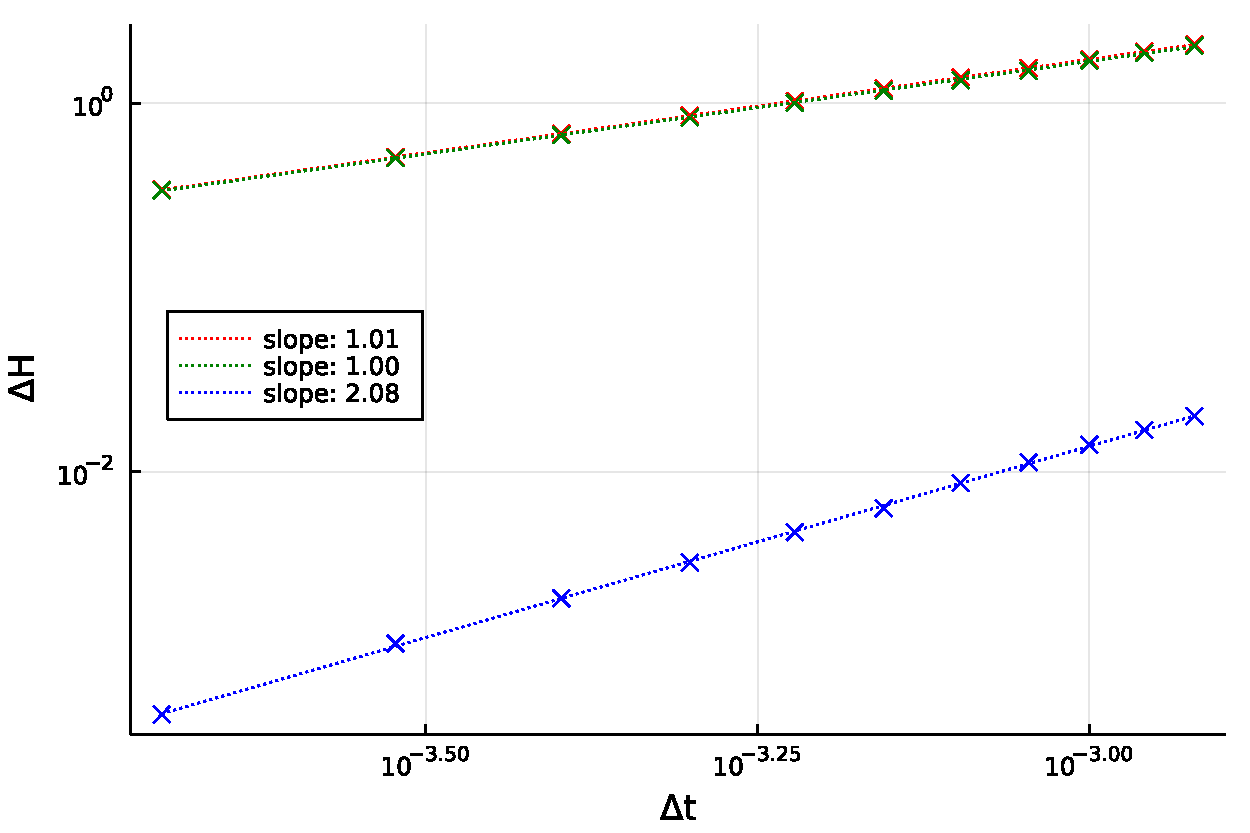
\includegraphics[width=0.7\linewidth]{figures/chapter1/hamiltonian_conservation.pdf}
          \caption{ \label{fig:hamiltonian_conservation}
            Effect of the time step on absolute variation of the Hamiltonian for the symplectic Euler (red and green) and the Verlet (blue) schemes. As expected, total variation scales as $\Delta t$ for symplectic Euler, and as $\Delta t^2$ for Verlet.
          }
        \end{center}
      \end{figure}
        
    \subsection{Shortcomings of the Hamiltonian approach}

\section{Canonical averages}

\subsection{Langevin dynamics}
We consider a special case of the inertial Langevin dynamics, defined by the following stochastic differential equation (SDE), where $\gamma, \beta$ are fixed positive constants.

\begin{equation}
    \label{eq:langevin}
    \left\{\begin{aligned}
        \text dq_t&=M^{-1}p_t\dt,\\
        \text dp_t&= -\nabla V(q_t)\dt -\gamma M^{-1}p_t\dt+\sqrt{\frac{2\gamma}\beta}\text dW_t,
    \end{aligned}\right.
\end{equation}

where $(W_t)_{t\geq 0}$ is a standard $dN$-dimensional Brownian motion.
This process is a combination of a Hamiltonian evolution with an additional action on the momenta which, if isolated, defines a $dN$-dimensional Ornstein-Uhlenbeck process.\\
This additional term be interpreted physically as the combination of two effects: a dissipation term 
$$-\gamma M^{-1}p_t\dt,$$
which can be understood as the effect of a viscous friction force on the particles, and a fluctuation term, 
$$\sqrt{\frac{2\gamma}\beta}\text dW_t,$$
which corresponds to the input of kinetic energy into the system as thermal agitation induced by a surrounding heat bath at temperature $1/(k_B\beta)$.\\
However, the physical meaning can be forgotten thanks to the fact that, \textit{in fine}, we only require that the canonical measure be invariant under this dynamic: as we shall shortly see, this is indeed the case.

\begin{remark}
    There are several ways to generalize this process: one is to consider more general, possibly non-separable, Hamiltonians, as in Remark \ref{rem:non_separable_hamiltonian}, rather than the classical Hamiltonian used above.
    The other is to allow the fluctuation-dissipation term to be parametrized by coefficients $\gamma$ and $\sigma$ depending on the state variable, and which obey a relation ensuring the invariance of $\mu$.
    Hence in full generality, we could consider the following Langevin dynamic:
    
    \begin{equation}
        \label{eq:general_langevin}
        \left\{\begin{aligned}
            \text dq_t &=\nabla_p H(q_t,p_t)\dt,\\
            \text dp_t &= -\nabla_q H(q_t,p_t)\dt -\gamma(q_t,p_t)\nabla_pH(q_t,p_t)\dt+\sigma(q_t,p_t)\rm{d}W_t.
        \end{aligned}\right.
    \end{equation}
\end{remark}
The generator of the Langevin dynamics is the operator
\begin{equation}
  \label{eq:langevin_generator}
\mathcal L_\gamma=M^{-1}p\cdot \nabla_q-\nabla V(q) \cdot \nabla_p- \gamma M^{-1} p \cdot \nabla_p+\frac\gamma\beta \Delta_p,
\end{equation}
which splits into three elementary generators, namely 
$$\mathcal L_\gamma= A+B+\gamma C=\cLham +\gamma C,$$
with
\begin{equation}
  \label{eq:C_definition}
C=-M^{-1}p\cdot \nabla_p +\frac1\beta \Delta_p.
\end{equation}
These generators individually give rise to dynamics which we can express explicitly, defined by the following evolution operators:

\begin{equation}
  \label{eq:propagators}
  \left\{\begin{aligned}
    &\mathrm{e}^{tA}\varphi(q,p)=\varphi(q+tM^{-1}p,p),\\
    &\mathrm{e}^{tB}\varphi(q,p)=\varphi(q,p-t\nabla V(q)),\\
   &\mathrm{e}^{t\gamma C}\varphi(q,p)=\mathbbm E \left[\varphi \left(q, \mathrm e^{-\gamma M^{-1}t}p + \sqrt{\frac{M}{\beta}(1-\mathrm{e}^{-2\gamma M^{-1}t})}G\right)\right],
\end{aligned}\right.
\end{equation}
where $G$ is a standard $dN$-dimensional Gaussian. The third equality translates an equality in law between an Itô integral and a Gaussian random variable, and follows by applying Itô's formula to the rescaled process
$$\e^{\gamma M^{-1}t}X_t,$$
where $X_t$ is the Ornstein-Uhlenbeck process:
\begin{equation}
    \dif X_t=-\gamma M^{-1}X_t\dif t+\sqrt{\frac{2\gamma}{\beta}}\dif W_t.
\end{equation}
 The dynamics associated with the A and B part are deterministic Hamiltonian dynamics already identified in \eqref{eq:Lham_splitting_dynamics_solved}.

\subsection{Properties of the Langevin dynamics}

    \subsubsection*{Invariance of the canonical measure}

    Using the generator, one can easily express the evolution of a probability distribution under the Langevin dynamics.
    We assume that the solution $(q_t,p_t)_{t\geq 0}$ to \eqref{eq:langevin} has a distribution with a smooth density $\rho_0$ over $\mathcal E$ at time $t=0$, and denote $\rho_t$ the probability density of $(q_t,p_t)$.
    For any test observable $\varphi$, we have
    $$\int_{\mathcal E}\varphi(q,p)\rho_t(q,p)\dif q\dif p=\int_{\mathcal E}\E^{(q,p)}\left[\varphi(q_t,p_t)\right]\rho_0(q,p)\dif q\dif p=\int_{\mathcal E}\mathrm{e}^{t\cL_\gamma}\varphi(q,p)\rho_0(q,p)\dif q\dif p,$$
    where the superscript is as in \eqref{eq:invariant_measure}. Thus,
    $$\frac{\partial}{\partial t}\int_{\mathcal E}\varphi(q,p)\rho_t(q,p)\dif q\dif p=\int_{\mathcal E}\mathrm{e}^{t\cL_\gamma}\cL\varphi(q,p)\rho_0(q,p)\dif q\dif p=\int_{\mathcal E}\cL_\gamma\varphi(q,p)\rho_t(q,p)\dif q \dif p$$
    If we define $\cL_\gamma^\dagger$ as the adjoint of $\cL_\gamma$ on the flat space $L^2(\mathcal E)$, that is,
    \begin{equation}
        \label{eq:L_dagger}
        \int_{\mathcal E}\cL_\gamma\varphi \psi=\int_{\mathcal E}\varphi \cL_\gamma^\dagger \psi \qquad\text{for all test functions }\phi,\,\psi,
    \end{equation}
    we have the Fokker-Planck equation,
    \begin{equation}\label{eq:fokker_planck}
        \frac{\partial}{\partial t}\int_{\mathcal E}\varphi(q,p)\rho_t(q,p)\dif q\dif p=\int_{\mathcal E}\varphi(q,p)\cL_\gamma^\dagger\rho_t(q,p)\dif q \dif p,
    \end{equation}
    which rewrites formally as 
    \begin{equation}
        \label{eq:fokker_planck_formal}
        \frac{\partial}{\partial t}\rho_t=\cL_\gamma^\dagger\rho_t.
    \end{equation}
    Using this equation, we can easily show that the canonical distribution is invariant under this dynamics, which is equivalent to the condition 
    $$\cL_\gamma^\dagger \mu=0.$$
    In fact, it is useful to reformulate this condition in the weighted space $L^{2}(\mu)$. Indeed, the stationary Fokker-Planck equation rewrites
    $$\int_{\mathcal E}\cL_\gamma \varphi \dif \mu=0\qquad \forall\,\varphi,$$
    or
    $$\int_{\mathcal E}\left(\cL_\gamma^* \1_{\mathcal E}\right)\varphi \dif \mu\qquad\forall\,\varphi,$$
    where $\cL_\gamma^*$ is the adjoint of $\cL_\gamma$ in $L^2(\mu)$ under the scalar product
    $$\langle \varphi,\psi \rangle_\mu\defeq \int_{\mathcal E}\varphi \psi \dif \mu.$$
    This, in turn, follows easily from the following lemma.
    \begin{lemma}
        \label{lemma:star_adjoints_langevin}
        The $L^2(\mu)$ adjoints of the elementary differential operators are given by the formulae
        \begin{equation}
            \label{eq:star_adjoints_langevin}
            \left\{\begin{aligned}
            &\partial_{q_i}^*=-\partial_{q_i}+\beta\partial_{q_i}V,\\
            &\partial_{p_i}^*=-\partial_{p_i}+\beta\left(M^{-1}p\right)_i.
            \end{aligned}\right.
        \end{equation}
    \end{lemma}
    These are easily found by integration by parts. In particular, we find that 
    $$\partial_{q_i}\partial_{p_i}^*-\partial_{p_i}\partial_{q_i}^*=\beta\left((M^{-1}p)_i\partial_{q_i}-\partial_{q_i}V\partial_{p_i}\right),$$
    whence, by summing over $i$, we get 
    \begin{equation}
        \label{eq:L_ham_antisymmetric}
        \cLham=\frac1\beta\left(\nabla_q\cdot\nabla_p^*-\nabla_p\cdot\nabla_q^*\right),
    \end{equation}
    which is an antisymmetric operator. Similarly,
    $$\partial_{p_i}\partial_{p_i}^*=\beta(M^{-1}p)_i\partial_{p_i}-\partial_{p_i}^2,$$
    hence
    \begin{equation}
        \label{eq:C_symmetric}
        C=-\frac{1}\beta\nabla_p\cdot\nabla_p^*,
    \end{equation}
    which is a symmetric operator. In summary, we have that 
    \begin{equation}
        \label{eq:L_star}
        \cL_\gamma^*=-\cLham+\gamma C=-(A+B)+\gamma C.
    \end{equation}
    It follows immediately that $\cL_\gamma^*\1_{\mathcal E}=0$. Notice that since $\cLham^*\1_{\mathcal E}=0$, the canonical measure is also invariant under the Hamiltonian dynamics. However, because of the energy conservation property \eqref{eq:energy_conservation}, ergodic averages cannot in general converge to their averages under $\mu$.

    \subsubsection{Convergence to equilibrium}

\subsection{Overdamped limit of Langevin dynamics}
    As already pointed out, the fact that the kinetic marginal of $\mu$ is a Gaussian distribution makes sampling canonical momenta trivial. 
    Instead, the main problem is sampling from $\nu$. It follows directly from the invariance of $\mu$ under trajectories of the Langevin dynamics that $\nu$ is invariant under the configurational trajectories of the Langevin dynamics.
    It would be convenient, however, to have at our disposal a dynamics on $\mathcal D$ which has $\nu$ as an invariant measure.
    It turns out this is possible, by observing that the invariance of $\mu$ is independent of the parameter $\gamma$, and taking the limit $\gamma\to\infty$. This requires some care.
    Notice the SDE on the momenta in \eqref{eq:langevin} rewrites 
    \[\dif p_t=-\nabla V(q_t)\dif t-\gamma \dif q_t+\sqrt{\frac{2\gamma}\beta}\dif W_t,\]
    thus integrating gives
    \[q_t-q_0=\frac{p_0-p_t}\gamma -\frac{1}\gamma\int_0^t\nabla V(q_s)\dif s +\sqrt{\frac{2}{\gamma\beta}}W_t.\]
    The scaling invariance of the Brownian motion $(\sqrt{\alpha}W_{t/\alpha^2})_{t\geq 0}\sim (W_t)_{t\geq 0}$ suggests considering the timescale $\gamma\beta t$, thus
    \[q_{\gamma\beta t}-q_0=\frac{p_0-p_{\gamma\beta t}}\gamma-\frac1{\gamma}\int_0^{\gamma\beta t}\nabla V(q_s)\dif s +\sqrt{2}\widetilde{W_t},\]
    where $\widetilde W$ is again a Brownian motion. Using the change of variables $s=\gamma \beta u$ in the integral term yields
    \begin{equation}\label{eq:rescaled_langevin}q_{\gamma\beta t}-q_0=\frac{p_0-p_{\gamma\beta t}}\gamma-\beta\int_0^{t}\nabla V(q_{\gamma\beta u})\dif u +\sqrt{2}\widetilde{W_t},\end{equation}
    At this point, we formally take $\gamma\to\infty$, which suggests the following SDE for the rescaled in time process,
    \begin{equation}
        \label{eq:overdamped_langevin}
        \dif q_t=-\beta \nabla V(q_t)\dif t+\sqrt{2}\dif W_t.
    \end{equation}
    
    This equation defines the overdamped Langevin, or Brownian, dynamics.
    To justify the limit in a rigorous manner, one would hope to show that the rescaled process \eqref{eq:rescaled_langevin} converges in law to a weak solution of the SDE \eqref{eq:overdamped_langevin}, in some functional space.
    However, this is technical overkill, since, we only need to consider dynamics as sampling devices. In fact, the physical interpretation of this equation is not even clear in terms of the dimensions of the quantities at play.
    We can just as well take equation \eqref{eq:overdamped_langevin} as given, and be satisfied by the following fact.

    \begin{prop}
        The configurational Gibbs measure $\nu$ is invariant under the dynamics \eqref{eq:overdamped_langevin}.
    \end{prop}

    This follows along the same lines as for the Langevin dynamics. The generator (now acting on observables defined on $\mathcal D$) is the operator
    \begin{equation}
        \label{eq:overdamped_langevin_generator}
        \cL\varphi=-\beta\nabla V\cdot \nabla\varphi + \Delta \varphi.
    \end{equation}
    Again, we consider the weighted space $L^2(\nu)$. Adjoints of elementary differential operators are still given by the first line of \eqref{eq:star_adjoints_langevin}, and it is then easily seen that
    \begin{equation}
        \label{eq:L_overdamped_symmetric}
        \cL=-\nabla^*\cdot\nabla
    \end{equation}
    is a symmetric operator. Again we have $\cL^*\1_{\mathcal D}=0$, so $\nu$ satisfies the stationary Fokker-Planck equation under this dynamics.

    \begin{remark}
        Instead of rescaling time by $\beta\gamma$, we could have rescaled by $\gamma$, which would yield the dynamics
        \begin{equation}
            \label{eq:overdamped_langevin_alt}
            \dif q_t=-\nabla V(q_t)\dif t+\sqrt{\frac 2\gamma}\dif W_t.
        \end{equation}
        Which formulation to choose is a matter of preference, since both yield a dynamics invariant under $\nu$, as seen from the identity (where we still write $\cL$ for the generator)
        \[\cL=-\frac1\beta\nabla^*\cdot\nabla.\]
    \end{remark}

    As for the Langevin dynamics, it is possible to show tha


\subsection{Splitting schemes for the Langevin dynamics}\label{section:splitting_schemes_langevin}
Just as in the Hamiltonian case, we can define schemes for the Langevin dynamics based on approximating the evolution operator over one timestep by splitting the generator $\cL_\gamma$, and combining the corresponding evolution operators \eqref{eq:propagators} in a sequence.
We refer to such a splitting approximation by the sequence in which the individual propagators are composed. It is useful at this point to introduce the stochastic flow map associated with the Ornstein-Uhlenbeck dynamics.
\begin{equation}
    \label{eq:stochastic_flow_c}
    \Phi_t^C(q,p,\xi)=\left(q, \mathrm e^{-\gamma M^{-1}t}p + \sqrt{\frac{M}{\beta}(1-\mathrm{e}^{-2\gamma M^{-1}t})}\xi\right),
\end{equation}
where $\xi\in \R^{dN}$, the point being $\E[\varphi\left(\Phi_t^C(q,p,G)\right)]=\mathrm{e}^{t\gamma C}\varphi(q,p)$ when $G$ is standard Gaussian.
Given an ordering of operators, 
\begin{equation}\label{eq:splitting_ordering}(R_1,\dots,R_k)\in \{A,B,\gamma C\}^k,\end{equation}
we can consider the mapping, which we note, by a slight abuse, as
\begin{equation}\label{eq:markov_mapping}\Phi^{R_1,\dots R_k}\defeq\Phi_{\Delta t/n_{R_k}}^{R_k}\circ\dots\circ\Phi_{\Delta t/n_{R_1}}^{R_1},
\end{equation}
where
$$n_R\defeq \#\left\{1\leq j\leq n \middle| R_j=R\right\}$$
for $R\in\{A,B,\gamma C\}$, and which we define to be the mapping which takes a point in phase space and $n_{\gamma C}$ vectors in $\R^{dN}$ $(\xi_1,\dots,\xi_{n_{\gamma C}})$, yielding a point in phase space by successively applying the flow, and, if need be, stochastic flow, mappings corresponding to the reverse ordering of \eqref{eq:splitting_ordering}.
Applying this mapping with a vector of independent standard Gaussians yields a stochastic mapping, which defines the update rule for the splitting scheme associated with the ordering \eqref{eq:splitting_ordering}.
An important property which follows from writing the update rule using the mapping \eqref{eq:markov_mapping} is that numerical trajectories formed by iterating this update rule with independent vectors of standard Gaussians form a Markov chain.
The hope is that the invariant measure corresponding to this Markov chain (provided it is unique) is a close approximation to the canonical measure, as well as being ergodic.

We will refer to such schemes by the name obtained by concatenating the names of each operator appearing in the ordering, using $O$ instead of $\gamma C$.
For instance, the BAO scheme is given by the following update rule, which corresponds to applying the symplectic Euler scheme over one timestep, followed by one timestep of the Ornstein-Uhlenbeck stochastic flow \eqref{eq:stochastic_flow_c}.

    \begin{example}[BAO scheme]
        The update rule is given by the following equations, where we introduce the intermediate momentum variable $p^{n+\frac12}$:
        \begin{equation}\label{bao}
            \left\{\begin{aligned}
                 p^{n+\frac12} &=p^n -\Delta t\nabla V(q^n)\\
                 q^{n+1} &=q^n + \Delta t M^{-1}p^{n+\frac 12}\\
                 p^{n+1} &= \alpha_{\Delta t}p^{n+\frac12}+\sigma_{\Delta t}G^n,
            \end{aligned}\right.
        \end{equation}
        where $G^n$ is a standard $dN$-dimensional Gaussian.
    \end{example}
    Similarly, we define the BAOAB scheme.
    \begin{example}[BAOAB scheme]
        The update rule is given by the following equations, with additional intermediate coordinate and momentum variables:
        \begin{equation}\label{baoab}
            \left\{\begin{aligned}
                 p^{n+\frac13} &=p^n -\frac{\Delta t}{2}\nabla V(q^n)\\
                 q^{n+\frac12} &=q^n + \frac{\Delta t}{2} M^{-1}p^{n+\frac 13}\\
                 p^{n+\frac23} &=\alpha_{\Delta t}p^{n+\frac13}+\sigma_{\Delta t}G^n\\
                 q^{n+1} &=q^{n+\frac12} + \frac{\Delta t}{2} M^{-1}p^{n+\frac 23}\\
                 p^{n+1} &= p^{n+\frac23}-\frac{\Delta t}{2}\nabla V(q^{n+1}),
            \end{aligned}\right.
        \end{equation}
        where, again, $G^n$ is a standard $dN$-dimensional Gaussian.
    \end{example}
     Now we have a recipe to make an infinite number of numerical schemes, which can easily be implemented in a computer.
     We could even go further and consider methods with an uneven distribution for the secondary timesteps, the introduction of negative secondary timesteps for the $A$ and $B$ steps, and so on.
     This room for creativity highlights the need for criteria to assess the quality of such schemes. Several considerations have to be weighed.

     \begin{enumerate}[(i)]
         \item Our aim is to compute long trajectories, which are needed to ensure that phase space is properly explored, as well as to obtain better statistical properties for averages \eqref{eq:discrete_ergodic_averages}. Thus, for a fixed computational budget, we desire a scheme which allows us to take as large a timestep $\Delta t$ as possible. This is the issue of numerical stability.
         \item The use of a positive timestep $\Delta t$ implies in general that the invariant measure for the Markov chain corresponding to a given scheme is not the canonical measure. This issue is called systematic error, or bias, and one would desire a scheme which minimizes this bias.
         \item The main computational cost in computing iterates of these numerical schemes is the evaluation of the gradient of the potential used for the $B$ steps. As such, it is desirable to have a scheme which requires as few evaluations of this gradient per iteration. Some care must be taken when implementing these, to ensure that already computed gradients are not re-computed: for instance, the gradient in the last step of the BOAB scheme, is equal to the one in the first step of the next iteration.
         \item Notice that the parameter $\gamma$ is free for the practicioner to choose. A natural question is to determine the properties of the marginal dynamics in $q$ in the limit $\gamma \to +\infty$, and in particular if we obtain a consistent discretization of the overdamped Langevin dynamics.
         \item Conversely, one could ask about properties of the dynamics as we take the Hamiltonian limit $\gamma\to 0$.
     \end{enumerate}

    \subsection{Error analysis for splitting schemes}
     Let us address the second of these concerns 

    \subsection{Unbiased sampling}
     It turns out that one can devise schemes which have no systematic error: the Markov chain generating the trajectories has invariant measure exactly $\mu$.
     These methods are based on the Metropolis-Hastings algorithm, which gives a general method to sample a given target distribution.
    \subsubsection*{The Metropolis-Hastings algorithm}
     We aim to sample from a given target measure on $\R^d$. We suppose we have at our disposal a way to generate proposal points from a given point $\in\R^d$. This amounts to defining a transition kernel, the \textit{proposal}, which we may take to be a map
     \[T:\R^d\times\R^d\longrightarrow\R_+,\]
     such that for any $x\in\R^d$, $T(x,\cdot)$ is a probability density on $\R^d$, and which is cheap to sample from (very often these are taken to be some form of Gaussian distribution). We also assume that we always have $T(x,y)>0$. (This is always the case if the kernel is Gaussian).
     We also fix a function $r:\R_+\to(0,1]$, the \textit{rule}, which satisfies the property
     \begin{equation}\label{eq:mh_rule}x\cdot r\left(\frac1x\right)=r(x)\end{equation}
     We then define a Markov chain by iterating the following algorithm, starting from an arbitrary point $q^0\in \R^d$.

     \begin{algorithm}[Metropolis-Hastings]
        From a given point $q^n$
        \begin{enumerate}[(1)]
            \item Sample a proposal $\tilde q^{n+1}$ according to the probability law $T(q^n,\cdot)$.
            \item Compute\[R(\tilde q^{n+1},q^n)=r\left(\frac{\pi(\tilde q^{n+1})T(\tilde q^{n+1},q^n)}{\pi(q^n)T(q^n,\tilde q^{n+1})}\right).\]
            \item With probability $R(\tilde q^{n+1},q^n)$, set $q^{n+1}=\tilde q^{n+1}$, otherwise, set $q^{n+1}=q^n$.
            \item Go back to step (1) with $q^n\leftarrow q^{n+1}$.
        \end{enumerate}
     \end{algorithm}

    Since $T$ defines a Markov chain, we may always write $\tilde q^{n+1}=\Phi(q^n,\xi^n)$ for some family of \iid variables $(\xi^n)_{n\geq 0}$. We can then write $q^{n+1}$ in a concise form:
    \begin{equation}
        \label{eq:metropolis_hastings_algorithm}
        q^{n+1}=\Phi(q^n,\xi^n)+\1_{U^n>R\left(\Phi(q^n,\xi^n),q^n\right)}\left(q^n-\Phi(q^n,\xi^n)\right)=\Psi(q^n,\xi^n,U^n),
    \end{equation}
    where the $U^n$ are \iid uniform on $[0,1]$, such that the $(\xi^n,U^n)$ are an independent family. This shows that the algorithm defines a Markov chain. Furthermore, we may compute
    \begin{equation}
        \begin{aligned}
            \pi(x)\mathbb P\left(q^1=y \middle| q^0=x\right)&=\pi(x)T(x,y)R(x,y)\\
            &=\pi(x)T(x,y)r\left(\frac{\pi(y)T(y,x)}{\pi(x)T(x,y)}\right)\\
            &=\pi(y)T(y,x)\frac{\pi(x)T(x,y)}{\pi(y)T(y,x)}r\left(\frac{\pi(y)T(y,x)}{\pi(x)T(x,y)}\right)\\
            &=\pi(y)T(y,x)r\left(\frac{\pi(x)T(x,y)}{\pi(y)T(y,x)}\right)\ \text{(Using \eqref{eq:mh_rule})}\\
            &=\pi(y)\mathbb P\left(q^1=x\middle|q^0=y\right).
        \end{aligned}
    \end{equation}
    Thus, the chain is reversible with respect to $\pi$ which is then is an invariant measure.
    Note that the algorithm is applicable even when we do not know how to evaluate $\pi$, but only the ratios $\pi(x)/\pi(y)$, which is in particular the case for Gibbs measures.

    \begin{remark}[Rules for Metropolis-Hastings]
        Possible choices for $r$ are:
        \begin{enumerate}
            \item The Metropolis rule, \[r(x)=\min\left\{1,x\right\},\]
            \item The Barker rule, \[r(x)=\frac{x}{1+x},\]
            \item Any combination of these of the form, for $\gamma>0$, \[r(x)=\frac{x}{1+x}\left(1+2\left(\frac12\min\left(r,\frac 1r\right)\right)^\gamma\right).\]
        \end{enumerate}
    \end{remark}

    \subsubsection*{Metropolized schemes for the underdamped Langevin dynamics}
    The Metropolis-Hastings algorithm provides a general recipe to define an unbiased Markov chain for the Langevin dynamics: one only needs to specify a proposition kernel and an acceptance rule.
    In fact, 

    \begin{example}[A GHMC scheme]
        Suppose we have at our disposal i.i.d families $(U_n)_{n\geq1}$ and $(G_n)_{n\geq 1}$ where $U_1$ is uniform on $[0,1]$ and $G_1$ is a standard Gaussian in $\R^{dN}$.
            \begin{equation}\label{ghmc}
                \left\{\begin{aligned}
                     &p^{n+\frac12} =\alpha_{\Delta t}p^n +\sigma_{\Delta t}G_n\\
                     &\tilde p^{n+\frac12} =p^{n+\frac 12} - \frac{\Delta t}{2} \nabla V(q^n)\\
                     &\tilde q^{n+1} =q^n+\Delta t M^{-1} \tilde p^{n+\frac 12}\\
                     &\tilde p^{n+1} =\tilde p^{n+\frac12} - \frac{\Delta t}{2} \nabla V(\tilde q^{n+1})\\
                     &r_n \defeq \min\left\{1,\exp(-\beta(H(\tilde q^{n+1},\tilde p^{n+1})-H(q^n,p^{n+\frac12})))\right\}\\
                     &(q^{n+1},p^{n+1}) = \1_{U_n > r_n}(q^n,-p^{n+\frac12})+\1_{U_n\leq r_n}(\tilde q^{n+1},\tilde p^{n+1})
                \end{aligned}\right.
            \end{equation}
        \end{example}

\subsection{Asymptotic variance}

\begin{figure}[htbp]
    \begin{center}
      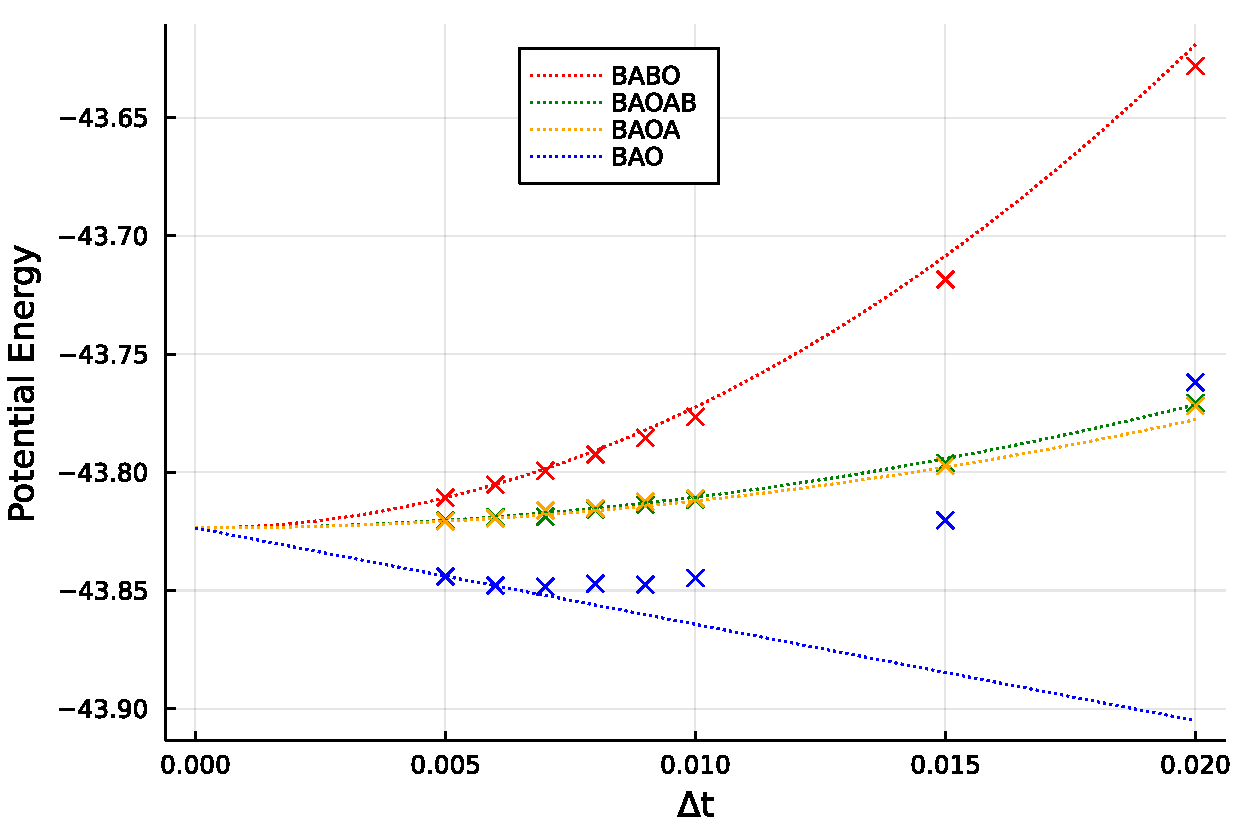
\includegraphics[width=0.49\linewidth]{figures/chapter1/potential_energy_bias.pdf}
      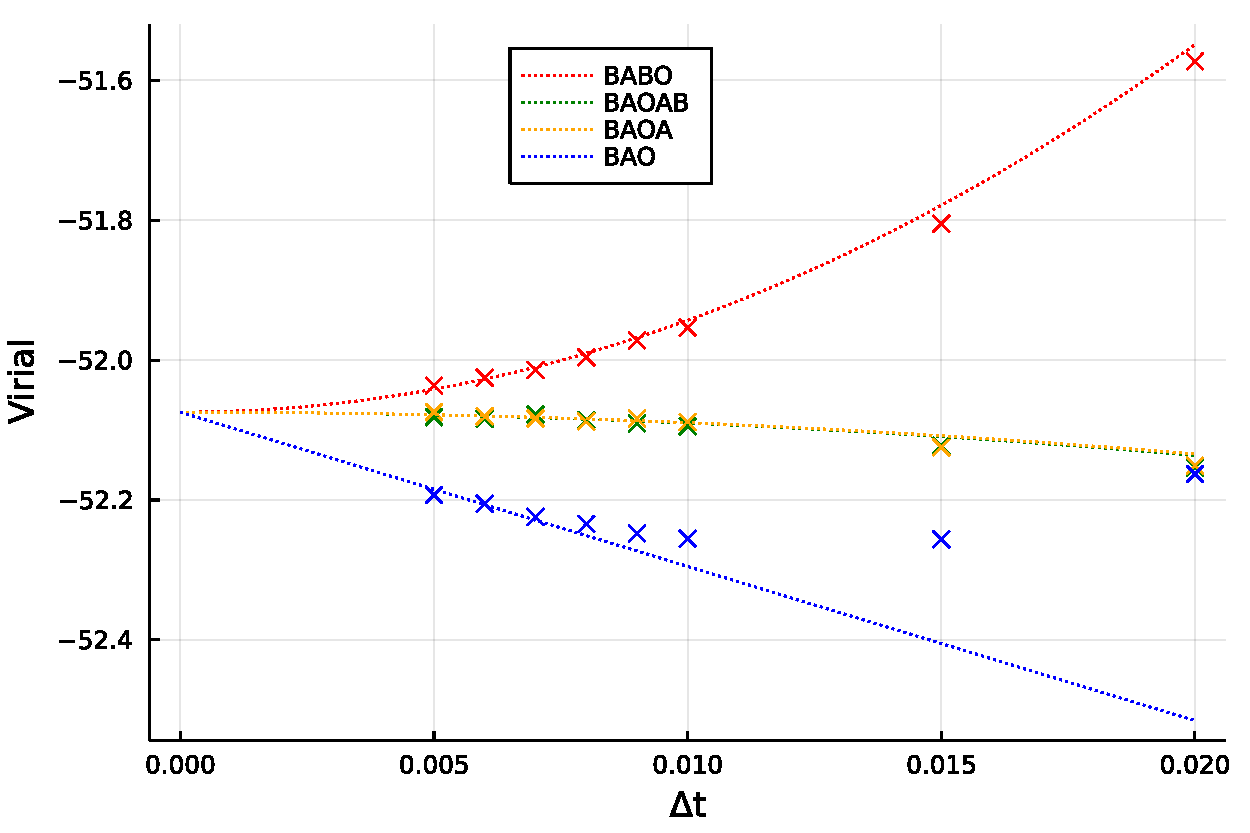
\includegraphics[width=0.49\linewidth]{figures/chapter1/virial_bias.pdf}
      \caption{ \label{fig:configurational_bias}
        Effect of the time step on average potential energy and virial for a Lennard-Jones system of 27 particles.
      }
    \end{center}
  \end{figure}

  \begin{figure}[htbp]
    \begin{center}
      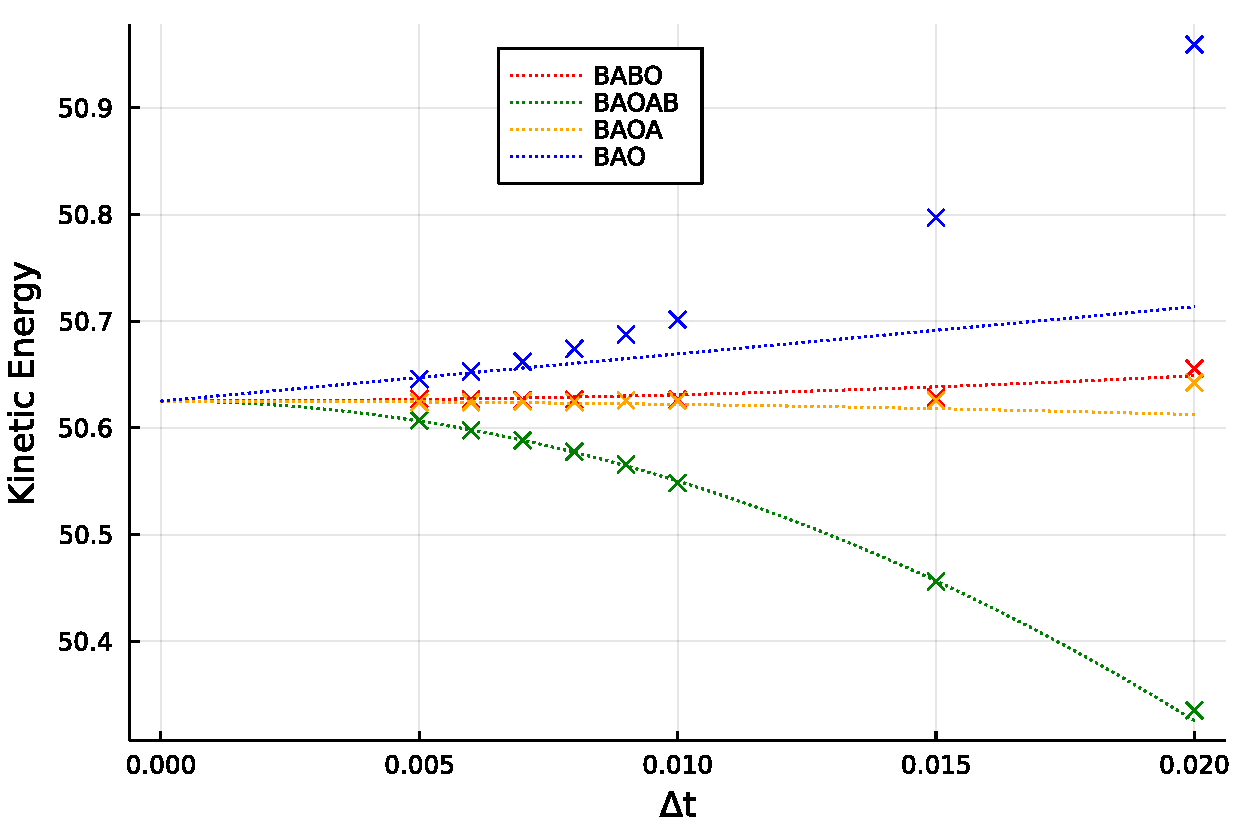
\includegraphics[width=0.7\linewidth]{figures/chapter1/kinetic_energy_bias.pdf}
      \caption{ \label{fig:kinetic_energy_bias}
        Effect of the time step on average kinetic energy for a Lennard-Jones system of 27 particles.
      }
    \end{center}
  \end{figure}

To explain the overlap of bias between the BAOAB and the BAOA schemes observed for the potential energy and virial on Figure \ref{fig:configurational bias}, we use the following result, which is a variation on the TU lemma.
\begin{lemma}\label{TU_like_lemma}
    Let $P_{\Delta t}, Q_{\Delta t}$ be bounded operators on $B^\infty(\mathcal E)$.
    Assume that, for any $n\geq 1$,
    $$ R P_{\Delta t}^n = Q_{\Delta t}^n S,$$
    where $R$ and $S$ are bounded operators on $B^\infty (\mathcal E)$, such that $R\1=\1$, and that the following ergodic condition holds: for any $\varphi \in B^\infty(\mathcal E)$, and almost all $(q,p) \in \mathcal E$,

    $$ \underset{n\to\infty}\lim P_{\Delta t}^n\varphi (q,p) = \int_{\mathcal E} \varphi(q,p)\mu_{\Delta t,P}(\text d q,\text d p) $$
    $$ \underset{n\to\infty}\lim Q_{\Delta t}^n\varphi (q,p) = \int_{\mathcal E} \varphi(q,p)\mu_{\Delta t,Q}(\text d q,\text d p).$$

    Then  we can relate $\mu_{\Delta t,P}$ and $\mu_{\Delta t,Q}$ via the following relation:

    \begin{equation}
        \label{TU_like_lemma_ccl}
    \int_{\mathcal E} \varphi(q,p) \mu_{\Delta t,P}(\text d q,\text d p)=\int_{\mathcal E} S\varphi(q,p) \mu_{\Delta t,Q}(\text d q,\text d p)
    \end{equation}
    \begin{proof}
        Fix an initial probability measure $\rho$ on $\mathcal E$, absolutely continuous with respect to the Lebesgue measure. Then we may write, using dominated convergence to pass to the limit:

        \begin{align*}
            &\int_{\mathcal E}RP_{\Delta t}^n \varphi(q,p)\rho(\text d q,\text d p)\\
            &=\int_{\mathcal E}P_{\Delta t}^n \varphi(q,p)R^{\dagger}\rho(\text d q,\text d p)\\
            &\underset{n\to\infty}{\longrightarrow}\int_{\mathcal E} \left(\int_{\mathcal E}\varphi(q,p)\mu_{\Delta t,P}(\text d q,\text d p)\right) R^\dagger \rho(\text d \tilde q,\text d \tilde p)\\
            &=\int_{\mathcal E}\varphi(q,p)\mu_{\Delta t,P}(\text d q,\text d p)\int_{\mathcal E}R\1 \text d \rho\\
            &=\int_{\mathcal E}\varphi(q,p)\mu_{\Delta t,P}(\text d q,\text d p)
        \end{align*}
        Furthermore, applying the ergodic condition to the bounded function $S\varphi$ gives

        $$ \int_{\mathcal E} Q_{\Delta t}^n (S\varphi)(q,p) \rho(\text d q,\text d p) \text d q \text d p \underset{n\to\infty}{\longrightarrow}\int_{\mathcal E} \left (\int_{\mathcal E}S\varphi(q,p)\mu_{\Delta t,Q}(\text d q,\text d p)\right)\rho(\text d \tilde q,\text d \tilde p)=\int_{\mathcal E}S\varphi(q,p)\mu_{\Delta t,Q}(\text d q,\text d p).$$

        Since $RP_{\Delta t}^n=Q_{\Delta t}^n S$, identifying the two limits yields \eqref{TU_like_lemma_ccl}
    \end{proof}
\end{lemma}

\begin{corollary}
Let $ \pi^{\mathrm{BAOA}}_{\Delta t}$ and $\pi^{\mathrm{BAOAB}}_{\Delta t}$ be the invariant measures for the Markov transition operators defined respectively by the BAOA and BAOAB schemes for a fixed timestep $\Delta t$. If the ergodic condition holds, then the corresponding marginal distributions on $\mathcal D$ are equal.

\begin{proof}
    We denote by $P_{\Delta t}$ the transition operator for the BAOA scheme, and similarly $Q_{\Delta t}$ for the BAOAB scheme. It is straightforward to check that 
    $$ \rme^{\frac{\Delta t}2 B}P_{\Delta t}^n=Q_{\Delta t}^n \rme^{\frac{\Delta t}2 B}.$$

    Assuming the ergodic condition of Lemma \ref{TU_like_lemma} (TODO reference article for sufficient conditions), we can apply the result to get, for any bounded measurable observable $\varphi$,

    $$ \int_{\mathcal E} \varphi(q,p)\pi^{\mathrm{BAOA}}_{\Delta t}(\text d q,\text d p)=\int_{\mathcal E} \rme^{\frac{\Delta t}2 B}\varphi(q,p)\pi^{\mathrm{BAOAB}}_{\Delta t}(\text d q,\text d p).$$

    Now if $\varphi (q,p)= \varphi (q,0) \defeq \varphi(q)$ for all $p$, then $\rme^{\frac{\Delta t}2 B}\varphi=\varphi$, which yields the desired conclusion:

    $$\forall \varphi \in B^\infty(\mathcal D),\ \int_{\mathcal E} \varphi(q)\pi^{\mathrm{BAOA}}_{\Delta t}(\text d q,\text d p)=\int_{\mathcal E}\varphi(q)\pi^{\mathrm{BAOAB}}_{\Delta t}(\text d q,\text d p).$$
\end{proof}

\end{corollary}

The corollary also gives a non-trivial relation between the marginal distributions in momentum space, which explains the difference displayed on (Figure \ref{fig:kinetic_energy_bias}) between those two schemes.



\subsection{Illustration: the equation of state of Argon}
\begin{figure}[htbp]
    \begin{center}
      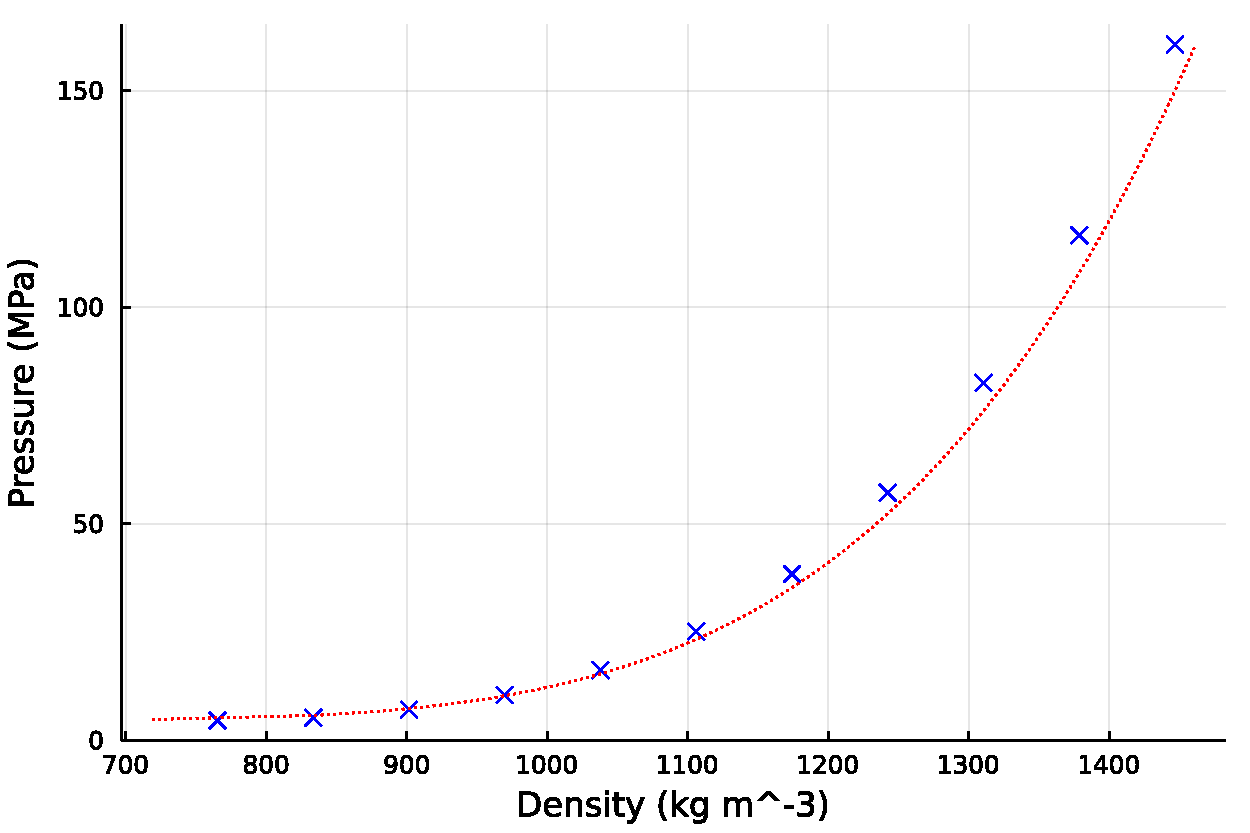
\includegraphics[width=0.49\linewidth]{figures/chapter1/argon_nvt_150K.pdf}
      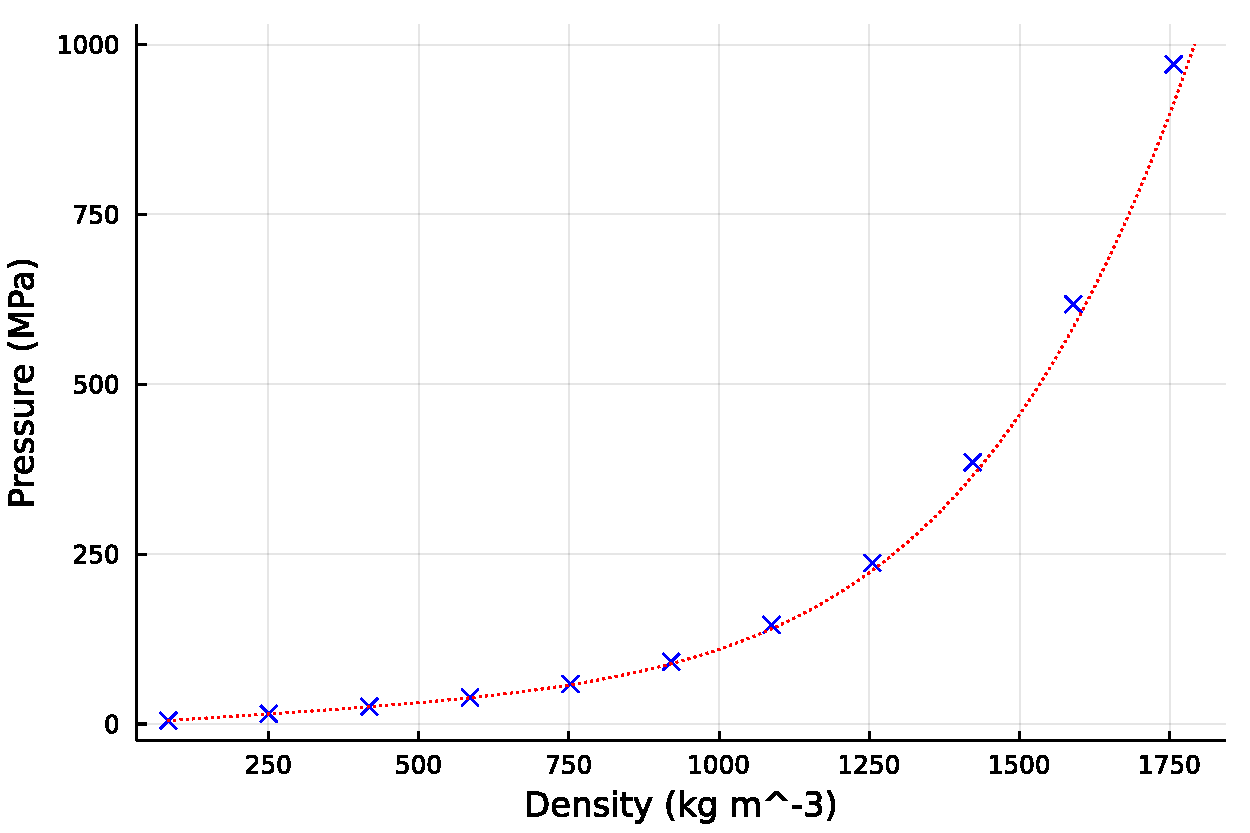
\includegraphics[width=0.49\linewidth]{figures/chapter1/argon_nvt_300K.pdf}
      \caption{ \label{fig:eos_argon}
        Simulated equations of state of Argon at 150 K (liquid phase, left) and 300 K (supercritical phase, right). Experimental reference curves are plotted in red, simulated data points are scattered in blue.
      }
    \end{center}
  \end{figure}